\documentclass{template}
\usepackage{tikz}
% 环绕
\usepackage{wrapfig}

\begin{document}
\ttfamily
\section{用于减少系统连接的复杂度}
如果我们有$ N $个不同的设备,且每个设备之间需要各自单独连接,
那么系统的复杂度就会变成$ N^2 $,引入总线后,复杂度就简化成$ N $.

与其让各个设备之间相互单独通信,不如去设计一个公用的线路,让各个设备都建一条通向这条主线路的线路就行了。



\section{总线仲裁 -- Bus Arbitration}
多个主设备同时竞争总线控制权时,需要以某种机制来选择一个主设备优先获得主线控制权,这个过程叫做\underline{仲裁},
且只有获得了总线控制权的设备,才能开始传送数据。

\begin{center}
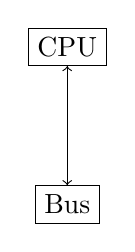
\begin{tikzpicture}
    % CPU node
    \node[rectangle, draw] (cpu) {CPU};
    
    % Bus node
    \node[rectangle, draw, below of=cpu, node distance=2cm] (bus) {Bus};
    
    % Arrows
    \draw[->] (cpu) -- (bus);
    \draw[->] (bus) -- (cpu);
  \end{tikzpicture}
\end{center}
\subsection{子标题}
\end{document}
